\section{A sufficiency criterion for retained state}\label{sec:C11:sufficiency}
The strongest justification for discarding history is that the retained representation preserves all information needed for the decisions being evaluated. Suppose $Y$ is a finite-valued target and $Z=\phi(H)$ is a deterministic state representation. Under logarithmic loss, the optimal expected losses using $Z$ and $H$ are $H(Y\mid Z)$ and $H(Y\mid H)$, respectively. Their difference is
\begin{equation}
 H(Y\mid Z)-H(Y\mid H)=I(Y;H\mid Z)\geq0.
 \label{eq:C11:informationloss}
\end{equation}
This is an information-theoretic deduction, not an empirical result about an existing agent. It assumes optimal conditional predictors and a fixed target distribution. Equality means that $Z$ is sufficient for predicting $Y$ relative to $H$. A fluent summary can have high semantic similarity to the original text while leaving this conditional mutual information strictly positive.

For sequential control, preserving the current answer is weaker than preserving future decisions. Let $X_t$ be the environment state and let $Z_t$ summarize observable history. A sufficient control state should support the conditional distribution of future observations and rewards under relevant action sequences. One possible exact condition is
\begin{equation}
 P(O_{t+1},R_t\mid H_t,a)=P(O_{t+1},R_t\mid Z_t,a)
\end{equation}
for every action under consideration, together with a recursively valid update of $Z_t$. This condition is demanding because the environment is partially observed and the action set may change when new tools become available. A task-oriented summary is usually an approximation to this condition rather than a demonstrated sufficient statistic.

Consider a repository task whose earlier history contains a requirement to preserve an undocumented compatibility behavior. A summary that retains the current implementation plan but omits that requirement may support the next edit and still fail a later regression check. The target variable in Eq.~\eqref{eq:C11:informationloss} must then include that later check. If evaluation asks only for the next action, the compression can appear lossless even though it removes information necessary for task completion. Horizon and target definition are part of any claim about retained information.

An approximate decision bound can be stated without assuming optimal language modeling. Suppose two histories represented by the same $z$ induce future-trajectory laws differing by at most $\epsilon\in[0,1]$ in total variation under every evaluated policy. For the same return functional $G$ taking values in $[-V_{\max},V_{\max}]$, their expected returns differ by at most $2V_{\max}\epsilon$. If instead $G\in[0,V_{\max}]$, the bound is $V_{\max}\epsilon$. These follow from the range of a bounded function and the definition of total variation. The observation motivates evaluating behaviorally distinct histories that collapse to the same summary. It does not provide a practical certificate unless the required uniform bound can be estimated or established from environment structure.

The engineering consequence is to make discarded distinctions explicit. Preserve obligations, authorization, unresolved alternatives, evidence provenance, and invalidated assumptions as typed state rather than relying on a generic narrative summary. Exact sufficiency may be unattainable, but the system can identify which future decisions its representation is intended to support and which distinctions it knowingly loses.

Information availability and a fixed model's competence must be separated when interpreting a full-history baseline. For a finite action space and bounded loss, define the Bayes risk under information $Z$ by
\begin{equation}
 R^*(Z)=\mathbb E\!\left[\min_a\mathbb E[\ell(a,Y)\mid Z]\right].
\end{equation}
If $Z=\phi(H)$, a policy with access to $H$ can imitate every $Z$-measurable decision rule, so $R^*(H)\leq R^*(Z)$. An observed improvement after deleting context therefore concerns the evaluated model, assembly procedure, and resource constraint; it does not show that removing information improves the unrestricted optimal decision. Compression can reduce distraction or make a finite computation feasible while still discarding information that another policy could use. This distinction is essential when attributing gains to a 2026 editor rather than to a weaker full-history implementation.



Figure~\ref{fig:C11:information-policy-risk} isolates the mechanism and its stated information boundaries.
\begin{figure}[!htbp]
\centering
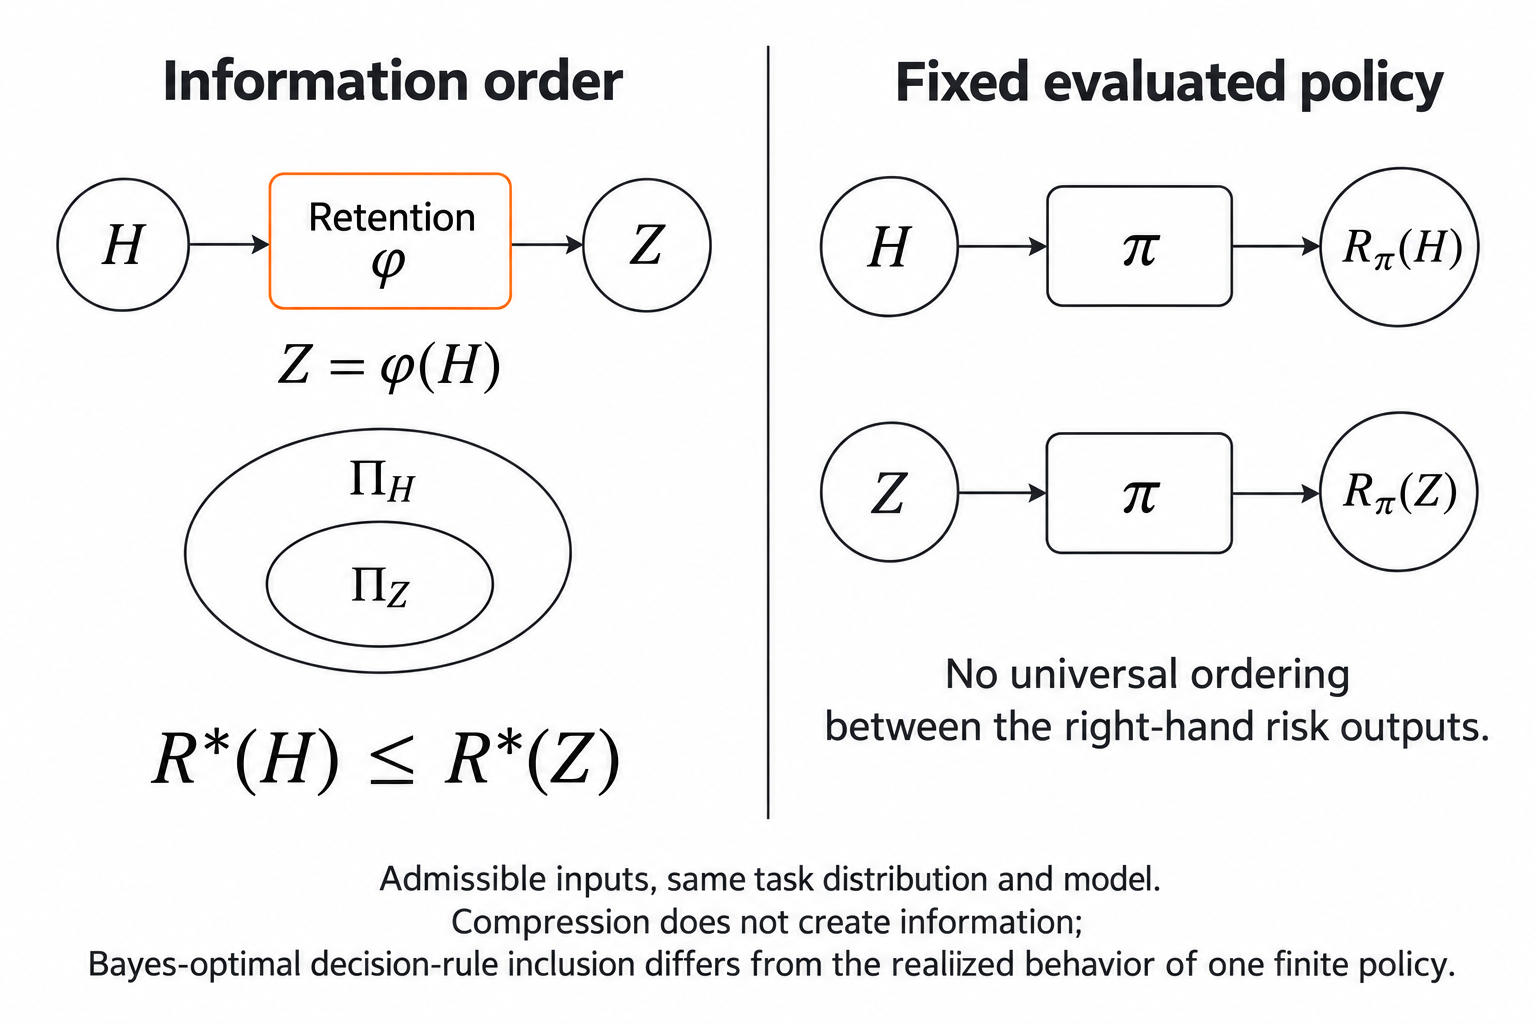
\includegraphics[width=\linewidth]{book/figures/assets/F11review.png}
\caption{Deterministic retention restricts the available decision rules, so $R^*(H)\leq R^*(Z)$ under the stated Bayes-risk assumptions. A fixed model can nevertheless perform better on a compressed view because computation, distraction and serialization affect its realized behavior. The right-hand risks have no universal ordering. This original schematic contains no empirical comparison.}
\label{fig:C11:information-policy-risk}
\end{figure}
